%%%%%%%%%%%%%%%%%%%%%%%%%%%%%%%%%%%%%%%%%
% Thin Sectioned Essay
% LaTeX Template
% Version 1.0 (3/8/13)
%
% This template has been downloaded from:
% http://www.LaTeXTemplates.com
%
% Original Author:
% Nicolas Diaz (nsdiaz@uc.cl) with extensive modifications by:
% Vel (vel@latextemplates.com)
%
% License:
% CC BY-NC-SA 3.0 (http://creativecommons.org/licenses/by-nc-sa/3.0/)
%
%%%%%%%%%%%%%%%%%%%%%%%%%%%%%%%%%%%%%%%%%

%----------------------------------------------------------------------------------------
%	PACKAGES AND OTHER DOCUMENT CONFIGURATIONS
%----------------------------------------------------------------------------------------

\documentclass[a4paper, 11pt]{article} % Font size (can be 10pt, 11pt or 12pt) and paper size (remove a4paper for US letter paper)

\usepackage[protrusion=true,expansion=true]{microtype} % Better typography
\usepackage{graphicx} % Required for including pictures
\usepackage{wrapfig} % Allows in-line images
\usepackage{caption}
\usepackage{subcaption}
\usepackage{booktabs}
\usepackage{tikz}
\usetikzlibrary{arrows,matrix,positioning}
\usepackage{multirow}
\usepackage{amsmath}
\usepackage{mathtools}
\usepackage{hyperref}
\usepackage{mathpazo} % Use the Palatino font
\usepackage[T1]{fontenc} % Required for accented characters
\linespread{1.05} % Change line spacing here, Palatino benefits from a slight increase by default

\makeatletter

\newcommand{\red}[1]{\textcolor{red}{#1}}
\newcommand{\ignore}[1]{}

\renewcommand\@biblabel[1]{\textbf{#1.}} % Change the square brackets for each bibliography item from '[1]' to '1.'
\renewcommand{\@listI}{\itemsep=0pt} % Reduce the space between items in the itemize and enumerate environments and the bibliography

\renewcommand{\maketitle}{ % Customize the title - do not edit title and author name here, see the TITLE block below
\begin{center} % Right align
{\LARGE\@title} % Increase the font size of the title

\vspace{50pt} % Some vertical space between the title and author name

{\large\@author} % Author name
\\\@date % Date

\vspace{40pt} % Some vertical space between the author block and abstract
\end{center}
}

%----------------------------------------------------------------------------------------
%	TITLE
%----------------------------------------------------------------------------------------

\title{\textbf{How our health makes us susceptible to COVID-19}\\ % Title
Springboard Capstone 2 Project} % Subtitle

\author{\textsc{Lisa Hahn-Woernle} % Author
\\{\textit{Data Scientist Bootcamp @ Springboard}}} % Institution

\date{\today} % Date

%----------------------------------------------------------------------------------------

\begin{document}

\maketitle % Print the title section

%----------------------------------------------------------------------------------------
%	ABSTRACT AND KEYWORDS
%----------------------------------------------------------------------------------------
\section{Introduction}
COVID-19 has changed the world as we know it. Airports, schools and offices closed. What seemed impossible is the new normal. But why are some countries hit more seriously than others? Culture, climate, social structures, health, ... these are just a few factors that can influence the spread of the disease. In this project, the susceptibility to COVID-19 and especially the fatalities due to COVID-19, is analyzed according to a country's health and demographics.

\section{Data}
\begin{figure}[htbp]
   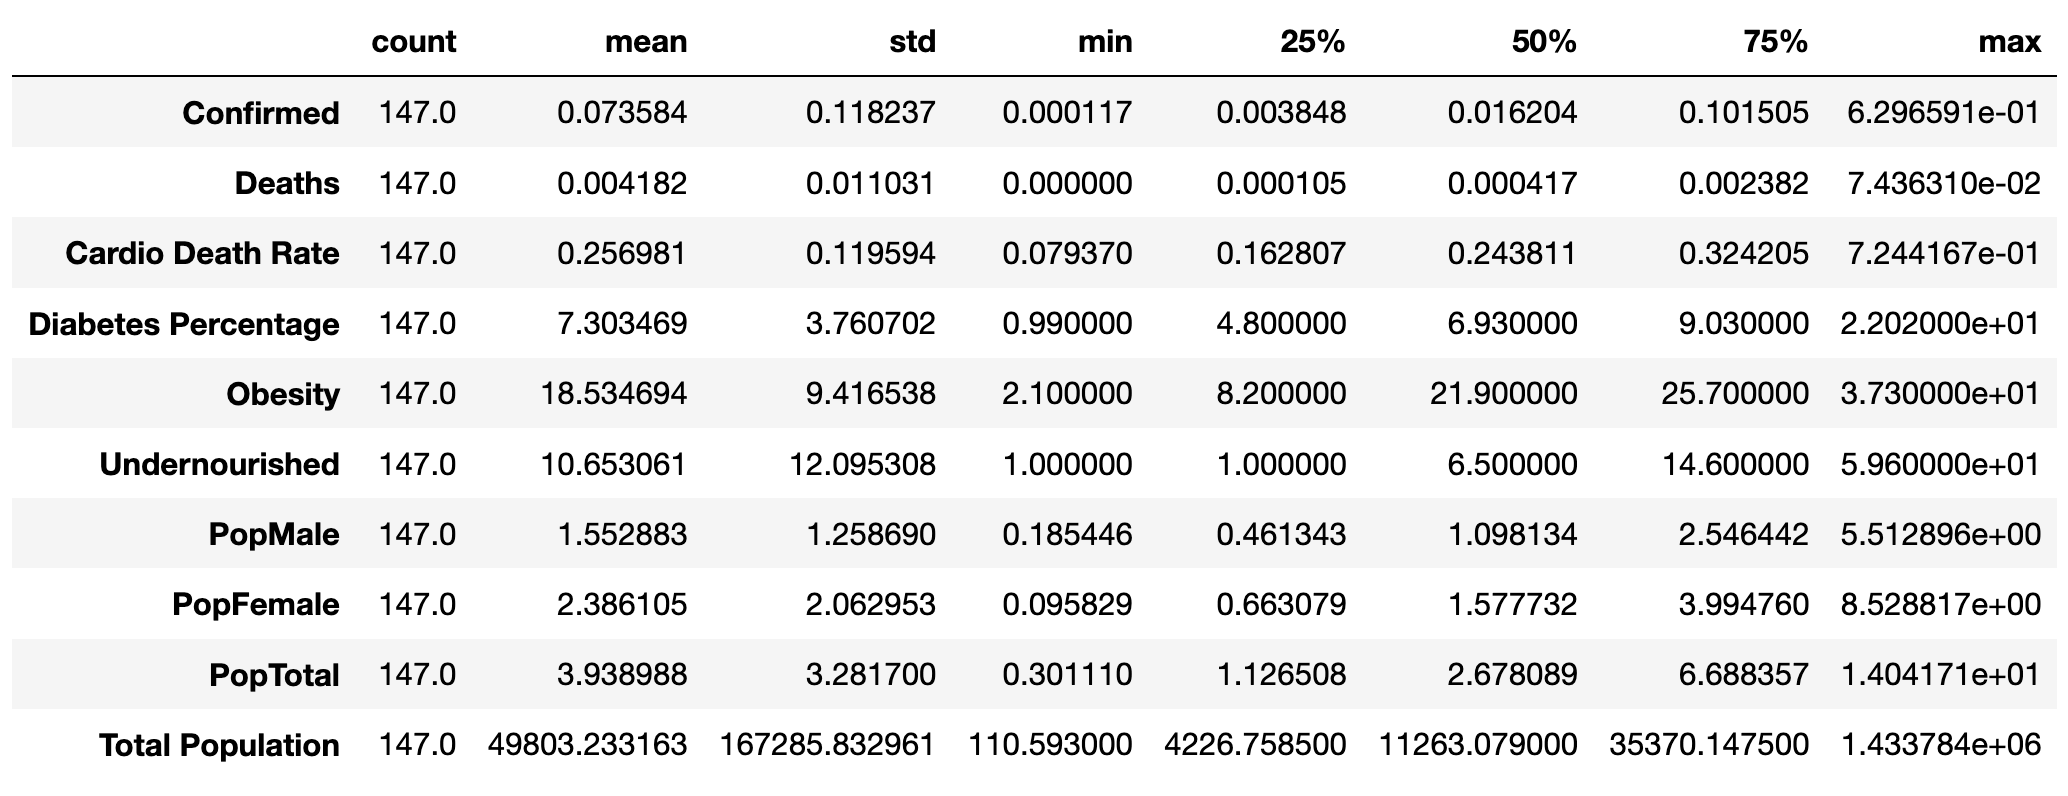
\includegraphics[width=0.9\linewidth]{figures/DataSet_Describe.png} 
   \caption{Properties of the numerical features in the COVID-19 data set. All features are relative to the Total Population (in thousand people).}
   \label{fig:Describe}
\end{figure}

\subsection{COVID-19 records}
The COVID-19 data is based on the COVID-19 Data Repository by the Center for Systems Science and Engineering (CSSE) at Johns Hopkins University on github (\url{https://github.com/CSSEGISandData/COVID-19}). The study is based on the global COVID-19 of May 9, 2020. While the notebooks could be reused for any other date, May 9, 2020 is the date this capstone project was first implemented.

The focus of this study is the mortality rate of the virus for a given country and its potential relationship to the national demographics and health statistics. Therefore, only the number of confirmed cases and of deaths are of interest to this study.

\subsection{Health records}
Here, the health of a nation is analyzed according to its most recent data of cardiovascular disease death rates, diabetes prevalence, and obesity and undernourishment rates. 

\textbf{Cardiovascular disease death rates} and \textbf{diabetes prevalence} are sourced from \url{ourworldindata.org} and are based on the 2017 statistics. \textbf{Obesity} and \textbf{undernourishment rates} are sourced from the Kaggle data set by Maria Ren (\url{https://www.kaggle.com/mariaren/covid19-healthy-diet-dataset}).

\subsection{Demographics}
Population size and gender-specific population percentages in the age group 75 and older are sourced from the UN population data set (\url{https://population.un.org/wpp}) for the year 2019.

\section{Method}
Data processing, analysis and modeling are all done with python in Jupyter Notebooks. If not stated differently, methods of the sklearn module are used.

First, the data set was reduced to the countries with COVID-19 cases. The resulting data set had no missing values and the only outlier was the US with its high number of confirmed COVID-19 cases. Second, the data set was scaled with the StandardScaler method and three clusters were derived with the KMeans method. The number of clusters was chosen based on the Elbow method. Third, the data was inspected with the Principal Component Analysis (PCA) method to verify the correctness of the clustering and visualize the data set in 2D. Fourth, the target, COVID-19 death rate, was separated from the data set, and both were split in a training (75 \%) and testing (25 \%) set. In the fifth and final step, the split data set was used to train and test different models: Linear Regression Model, Decision Tree Regressor, Random Forest Regressor, and Gradient Boosting Regressor. As performance measure the $R^2$ value and the mean squared error (MSE) are used.

\begin{figure}[htbp]
%\begin{subfigure}{0.45\textwidth}
%\centering
   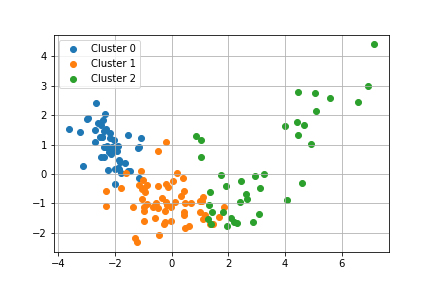
\includegraphics[width=0.9\linewidth]{figures/PCA_Clusters.png} 
%  \end{subfigure}
%     \begin{subfigure}{0.45\textwidth}
%  \centering
%   \includegraphics[width=0.9\linewidth]{../Figures/MeltwaterSeason.png} 
%  \end{subfigure}
%% requires the graphicx package
   \caption{Projection of the 11-dimensional dataset onto the 2 main components of the principal component analysis with the color coding according to the 3 clusters determined with the KMeans method.}
   \label{fig:PCA}
\end{figure}

\subsection{Motivation of Model Choice}
The key question of this project focusses rather on the feature importance than on the predictive power of a model. Still, the predictive power is seen as a measure on how reliable the choice of features and their importance are. The \textbf{2nd degree polynomial regression model} (2dPRM) is the result of a \textit{GridSearchCV} hyperparameter tuning step which was motivated by the polynomial shape of the PCA (Fig.~\ref{fig:PCA}). While the 2dPRM is cheap and easy to understand, it is clearly limited to the polynomial relation of the underlying data and is also prone for overfitting. Therefore, the other three models are based on the decision tree principle, which does not rely on linear or polynomial relations among features. To start off, the simple \textbf{Decision Tree Regressor} is used since it is easier to understand than the other, more complex models like the \textbf{Random Forest Regressor}. Random Forests, as the name says, rely on an ensemble of randomly selected decision trees. This makes the model more accurate and less prone to overfitting. The \textbf{Gradient Boosting Regressor} is similarly structured as the Random Forest, but learns from each decision tree to improve the next. While this can lead to more accurate results, overfitting might again become an issue. 

For all models, but especially the latter two ones, the small data set, with its 147 countries and 9 features, might limit the predictive power. Still, the choice of models provides insight from two different angles: one with a classical regression model and three different approaches using more abstract and modern machine learning techniques.

\subsection{2nd Degree Polynomial Regression Model (2dPRM)}
For the linear regression modeling the data is preprocessed with the PolynomialFeatures method to describe the data as a second order polynomial function (without bias). Based on the \textit{GridSearchCV} method, the 2nd degree polynomial was found to have the best predictive power. A 2nd degree polynomial is described as follows:
\begin{equation}
f(\vec{x}) = \sum_{i,j}^{N(i\leq j)} [a_{i,j}\cdot x_i \cdot x_j] + \sum_{i}^{N} [b_i \cdot x_i ]+ c \; ,
\label{eq:Poly}
\end{equation}
where $N$ is the number of features $x$ and the coefficients $a$ ($\frac{1}{2}N[N+1]$), $b$ ($N$) and $c$ (1) are determined during the fitting procedure.

\subsection{Decision Tree Regressor (DTR)}
Tuning with the GridSearchCV method lead to the following parameters for the Decision Tree Regressor: max\_depth = 3, max\_features = 6, min\_samples\_leaf = 3. All other parameters remained at their default value.

\subsection{Random Forest Regressor (RFR)}
The RandomForestRegressor was tuned to 250 estimators and all other parameters were left at their default values.

\subsection{Gradient Boosting Regressor (GBR)}
Based on a GridSearchCV tuning analysis, the following parameters for the GradientBoostingRegressor were set: max\_depth = 3, max\_features = 3, and n\_estimators = 150.

\section{Results}
The goal of the modeling is to identify i) whether a relationship between the COVID-19 fatalities and the health statistics and demographics data exists, and ii) which features are most relevant for the prediction of COVID-19 fatalities.

\subsection{Model Performance}

Table \ref{tab:ModelResults} lists the performance for all regression models as described in the method section. The Polynomial Regression Model has the best predictive power as measured with $R^2$ and MSE. While the Gradient Boosting Regressor is faster in prediction, the difference is so too small to make an argument for the weaker performing model. The Decision Tree performs the worst which stresses that the ensemble method improves the predictability and reduces the risk of overfitting.

\begin{table}[htbp]
\small
   \centering
   %\topcaption{Table captions are better up top} % requires the topcapt package
   \begin{tabular}{@{} l | c c c c @{}} % Column formatting, @{} suppresses leading/trailing space
      \toprule
      Model & $R^2$ & MSE& time fit [ms] &time predict [ms] \\
\midrule
Polynomial Regression &0.7643 & 0.6030  & 14.1 &3.1 \\
Decision Tree & 0.6088 & 1.001 & 34.6 & 9.4\\
Random Forest & 0.7173 & 0.7233 &520 & 26.4 \\
Gradient Boosting & 0.6961 & 0.7778 &87.8 &1.7 \\
 \bottomrule
   \end{tabular}
   \caption{$R^2$, mean squared error (MSE) and computation costs for the different models used in the analysis.}
   \label{tab:ModelResults}
\end{table}

\subsection{Feature Importance} 

The six largest coefficients (positive and negative) of the trained Polynomial Regressor based on Equ.~\ref{eq:Poly} are given as:

\begin{align}
f(x) = \; & \text{Cluster}_2 \cdot \begin{pmatrix} +1.28 \;\text{Undernourished} \\\nonumber
-1.15\;\text{Confirmed}\\
-0.79\;\text{Male}_{75+}\\
-0.62\;\text{Diabetes}\end{pmatrix}\\
&+\text{Confirmed}\cdot\begin{pmatrix}+0.72\;\text{Male}_{75+}\\ +0.79\end{pmatrix} + ... \; .
\label{eq:Poly_fit}
\end{align}
This result clearly identifies the number of confirmed COVID-19 cases and of males of age 75 and older as a key feature for the modeling. Further more, $Cluster 2$ appears to bear relevant information.

\begin{figure}[htbp]
\centering 
   \includegraphics[width=0.9\linewidth]{figures/DecisionTree.png} 
   \caption{Setup of the trained decision tree with a maximum depth of 3 and a minimum leaf size of 3.}
   \label{fig:DT}
\end{figure}
Figure~\ref{fig:DT} shows the trained setup of the Decision Tree. The setup already visualizes the dominant importance of the confirmed COVID-19 cases (76.3 \%), and the lower importance of diabetes (22.3 \%) and the male population older than 75 (1.4 \%). Even though the feature number was only limited to 6, the model actually relies on just 3.


Both the Random Forest and the Gradient Boosting Regressor provide the feature importance as a percentage in relationship to all features (Fig.~\ref{fig:Pies}). As could have been expected, for both models the number of confirmed COVID-19 cases is the most important feature. The RFR is dominated by this feature (74.5 \% for the confirmed cases), followed by Diabetes (9.1 \%) and male population older than 75 (7.1 \%). Obesity (3.1 \%) and cardiovascular death (2.4 \%) rank 5th and 6th after the total population size (3.2 \%) (Fig.~\ref{fig:Pies})a.). 

In the GBR, the confirmed cases make up only 41.2 \%. The male population older than 75 (20.5 \%) and Diabetes (13.4 \%) are again in the top 3, but in reverse order than in the RFR. Rank 4 is again the total population size (8.5 \%), followed by the cardiovascular death (6.2 \%) and obesity (5.4 \%). The latter are again in the reverse order compared to the RFR. Undernourishment appears to be not suited as indicator for the fatality of COVID-19 (RFR: 0.4 \%, GBR: 1.8 \%) (Fig.~\ref{fig:Pies})b.).

Figure~\ref{fig:Scatter} shows the relationship between the death rate and the top 4 important features according to RFR and GBR. Generally speaking, there is no strong trend in the data but higher death rates occur more likely in nations with more confirmed cases, more males older than 75, and a larger population. Cluster \#2 appears to contain countries with high fatalities, many confirmed cases, and the largest male population older than 75. Cluster \#0 contains countries with Diabetes cases and a small male population older than 75+.

\begin{figure}[htbp]
%\begin{subfigure}{0.45\textwidth}
%\centering
   \includegraphics[width=\linewidth]{figures/Scatter_Top4.png} 
%  \end{subfigure}
%     \begin{subfigure}{0.45\textwidth}
%  \centering
%   \includegraphics[width=0.9\linewidth]{../Figures/MeltwaterSeason.png} 
%  \end{subfigure}
%% requires the graphicx package
   \caption{Relationship between the death cases and i) confirmed cases, ii) male population (>75), iii) Diabetes (logarithmic x-scale), and iv) total population (logarithmic x-scale).}
   \label{fig:Scatter}
\end{figure}

\begin{figure}[htbp]
\begin{subfigure}{0.5\textwidth}
\centering 
   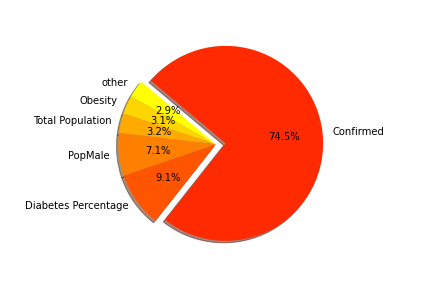
\includegraphics[width=\linewidth]{figures/Pie_RandomForest.png} 
   a. Random Forest
  \end{subfigure}
     \begin{subfigure}{0.5\textwidth}
  \centering
   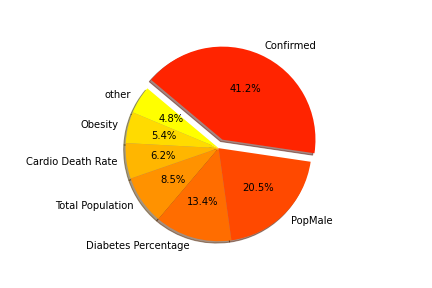
\includegraphics[width=\linewidth]{figures/Pie_GradientBoosting.png} 
     b. Gradient Boosting
  \end{subfigure}
% requires the graphicx package
   \caption{Feature importance based on the training of the two regression models.}
   \label{fig:Pies}
\end{figure}


\section{Conclusions and Recommendations}

The data analysis and modeling has revealed that next to the number of confirmed cases the percentage of the population that is male and older than 75, and the diabetes rate of a nation correlates to the fatality of COVID-19. Whether this is due to the effect of COVID-19 on elderly males and diabetes patients, or rather due to the fact that wealthier countries have higher diabetes rates and an older population, cannot be determined from this data set. But since obesity is also a sickness of the wealthy people, and since obesity ranks low, it is still very likely that elder males and diabetes patients are more susceptible to COVID-19 compared to the rest of the population.

Based on this study, it is recommended to particularly protect the male elderlies and diabetes patients from contact with the COVID-19 virus until a cure or vaccination has been found. Further analysis is needed to determine to which degree these two features represent wealthy countries  and to which degree the correlation is purely health related. Additionally, more recent data should be analyzed since it will extend the data set to more nations, unfortunately, including more developing countries. This shift in the distribution could lead to different modeling results and hence different feature importances.


\end{document}